\documentclass[tikz]{standalone}
\usepackage{xcolor}
\usetikzlibrary{mindmap} %for mindmap
\definecolor{DeepSkyBlue4}{RGB}{0,104,139}
\begin{document}
\tikzstyle{level 2 concept}+=[sibling angle=40]
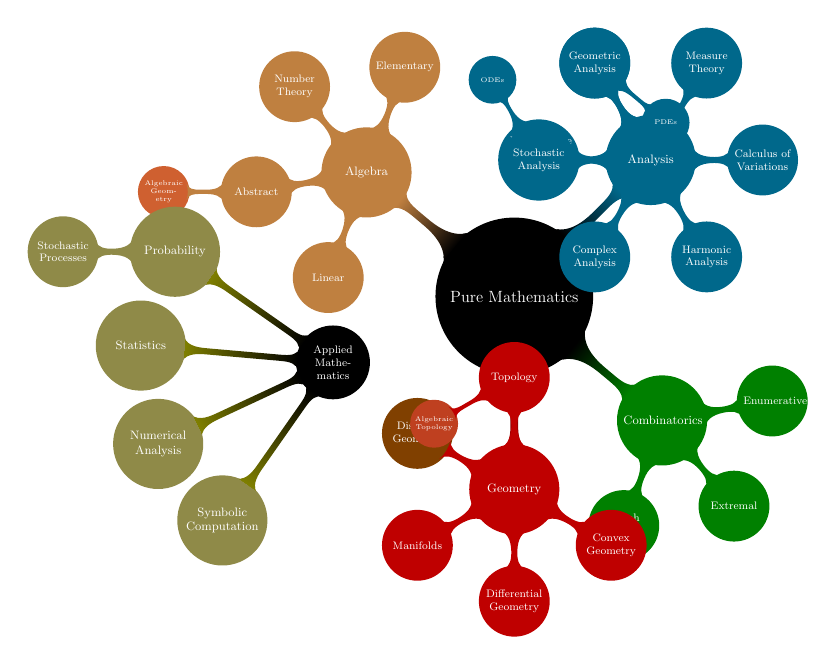
\begin{tikzpicture}[scale=0.49, transform shape]
\path[mindmap,concept color=black,text=white]
node[concept] {Pure Mathematics} [clockwise from=45]
child[concept color=DeepSkyBlue4]{
node[concept] {Analysis} [clockwise from=180]
child {
node[concept] {Multivariate \&amp; Vector Calculus}
[clockwise from=120]
child {node[concept] {ODEs}}}
child { node[concept] {Functional Analysis}}
child { node[concept] {Measure Theory}}
child { node[concept] {Calculus of Variations}}
child { node[concept] {Harmonic Analysis}}
child { node[concept] {Complex Analysis}}
child { node[concept] {Stochastic Analysis}}
child { node[concept] {Geometric Analysis}
[clockwise from=-40]
child {node[concept] {PDEs}}}}
child[concept color=black!50!green, grow=-40]{
node[concept] {Combinatorics} [clockwise from=10]
child {node[concept] {Enumerative}}
child {node[concept] {Extremal}}
child {node[concept] {Graph Theory}}}
child[concept color=black!25!red, grow=-90]{
node[concept] {Geometry} [clockwise from=-30]
child {node[concept] {Convex Geometry}}
child {node[concept] {Differential Geometry}}
child {node[concept] {Manifolds}}
child {node[concept,color=black!50!green!50!red,text=white] {Discrete Geometry}}
child {
node[concept] {Topology} [clockwise from=-150]
child {node [concept,color=black!25!red!50!brown,text=white]
{Algebraic Topology}}}}
child[concept color=brown,grow=140]{
node[concept] {Algebra} [counterclockwise from=70]
child {node[concept] {Elementary}}
child {node[concept] {Number Theory}}
child {node[concept] {Abstract} [clockwise from=180]
child {node[concept,color=red!25!brown,text=white] {Algebraic Geometry}}}
child {node[concept] {Linear}}}
node[extra concept,concept color=black] at (200:5) {Applied Mathematics}
child[grow=145,concept color=black!50!yellow] {
node[concept] {Probability} [clockwise from=180]
child {node[concept] {Stochastic Processes}}}
child[grow=175,concept color=black!50!yellow] {node[concept] {Statistics}}
child[grow=205,concept color=black!50!yellow] {node[concept] {Numerical Analysis}}
child[grow=235,concept color=black!50!yellow] {node[concept] {Symbolic Computation}};
\end{tikzpicture}
\end{document}
